\chapter{O Seu Objetivo}

\begin{center}
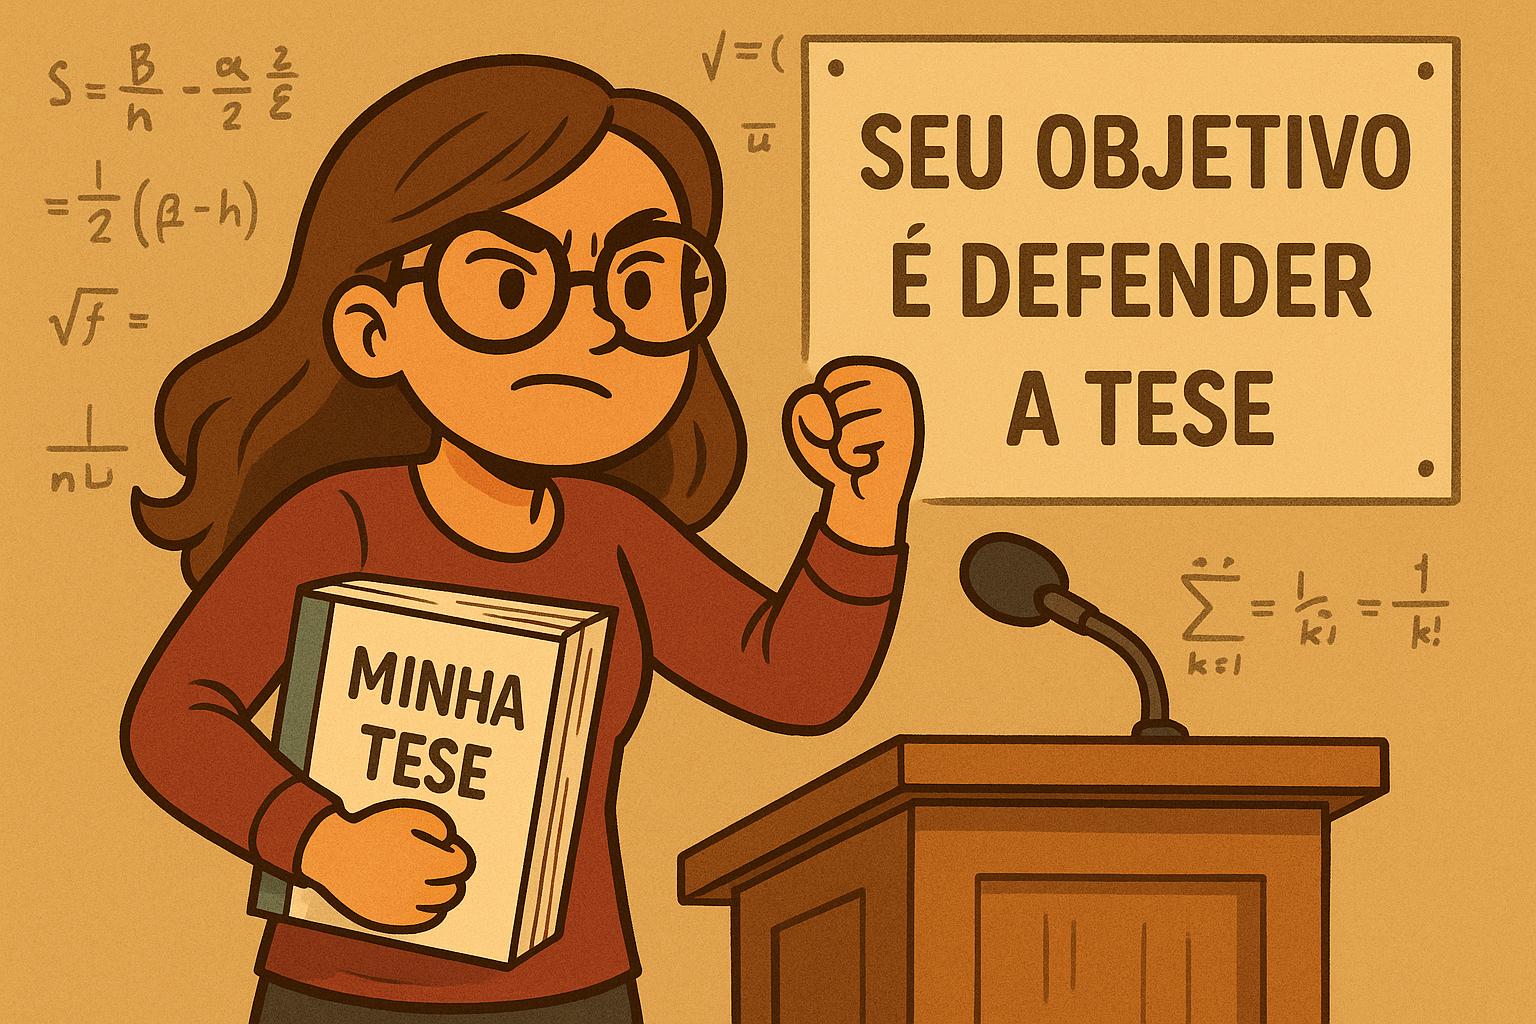
\includegraphics[width=0.5\linewidth]{Images/defender.png}    
\end{center}
\vspace{0.5cm}


Vamos deixar bem claro:

\gxatencao{O seu objetivo é defender a tese!}

Uma tese \textbf{não} é um trabalho completo que vai dar a melhor solução do mundo para o problema mais importante que existe.

Na Coppe, uma tese tem objetivos definidos da seguinte forma :
\begin{itemize}
\item	``A Dissertação de Mestrado deverá demonstrar a aptidão do candidato para desenvolver atividades de pesquisa no tema escolhido e configurar uma contribuição significativa para o conhecimento na área correspondente''
\item	``A Tese de Doutorado deverá apresentar características de originalidade, demonstrando a aptidão do candidato para desenvolver atividades de pesquisa, e configurar uma contribuição significativa para o conhecimento nas áreas escolhidas de pesquisa''
\end{itemize}

Ou seja, sua tese tem que ser uma \textbf{contribuição} para a área e, no caso do Doutorado, apresentar características de originalidade. É comum, no PESC, que uma tese de mestrado já apresente essas características, mas não é necessário.

Além disso, sua tese deve \textbf{acabar dentro do prazo}.

Alguns ditados que recolhi entre amigos orientadores e orientados deixam bem clara a importância de terminar a tese:

\begin{center}
``Tese não se termina, se entrega.''

``Tese boa é tese que acaba.''

``Você quer salvar o mundo ou tirar o título?''
    
\end{center}

Essas, e outras variações, são necessárias porque é comum o autor da tese achar que precisa ``resolver o problema do mundo'' ou que deve fazer uma tese perfeita. Isso é impossível, pois a tese está limitada em tempo.

Uma característica importante sobre teses de Doutorado: ao contrário do que muitos alunos pensam, uma tese que deixe muitos caminhos abertos é muito boa. Se isso acontece, o novo doutor é capaz de construir sua carreira, pelo menos inicialmente, resolvendo os problemas que ele mesmo descobriu ou tornou solucionáveis.

A professora Ana Regina Cavalcanti da Rocha costuma dizer:

\gxatencao{A Tese de Doutorado não é o último trabalho da vida de aluno, mas sim o primeiro trabalho da vida de pesquisador.}



